\chapter{Introduction}
The loss of muscle mass with aging and disuse atrophy has been studied extensively. 
Accompanying the loss of muscle mass (\textit{sarcopenia}) is a disproportionately greater loss of muscle strength (\textit{dynapenia}) as we age~\cite{RNIGoodpaster}. 
Sarcopenia and dynapenia will soon affect in excess of 50 million people worldwide with an increasingly aging population. 
The morbidity associated with loss of muscle quality and strength makes this a clinical problem of high significance. 
Muscle quality is multifactorial and a comprehensive evaluation of all factors is required to understand its decrease with age and disuse. Among these factors, the role of muscular and neural determinants of muscle force have been investigated in several human and animal studies~\cite{RNIBallak}.
In addition to these determinants, the role of the extracellular matrix is also being increasingly recognized~\cite{RNIRamaswamy, RNIZhang}. 
For example, aging significantly alters proteins that transmit force both inside the muscle fibers~\cite{RNIHughes} and in the extracellular matrix~(ECM)~\cite{RNIKragstrup}, changing their content, orientation and composition. 
The remodeling of the ECM may also contribute to muscle weakness by impairing a muscle's capacity to transmit force. 
For example, in young rodent muscles, at least 80\% of force transmission occurs laterally through the ECM~\cite{RNIHuijing}, whereas in frail old muscle, lateral transmission of force (LTF) through the ECM is reduced ~60\%~\cite{RNIRamaswamy, RNIZhang}. 
However, the contribution of the ECM to \textit{dynapenia} has never been comprehensively investigated in humans due to lack of non-invasive tools.
%-new paragraph-%

%-new paragraph-%
A brief overview of muscle anatomy and physiology is provided to set the context for the dissertation. 
%*********************************************************
\begin{figure}[!ht]
\centering
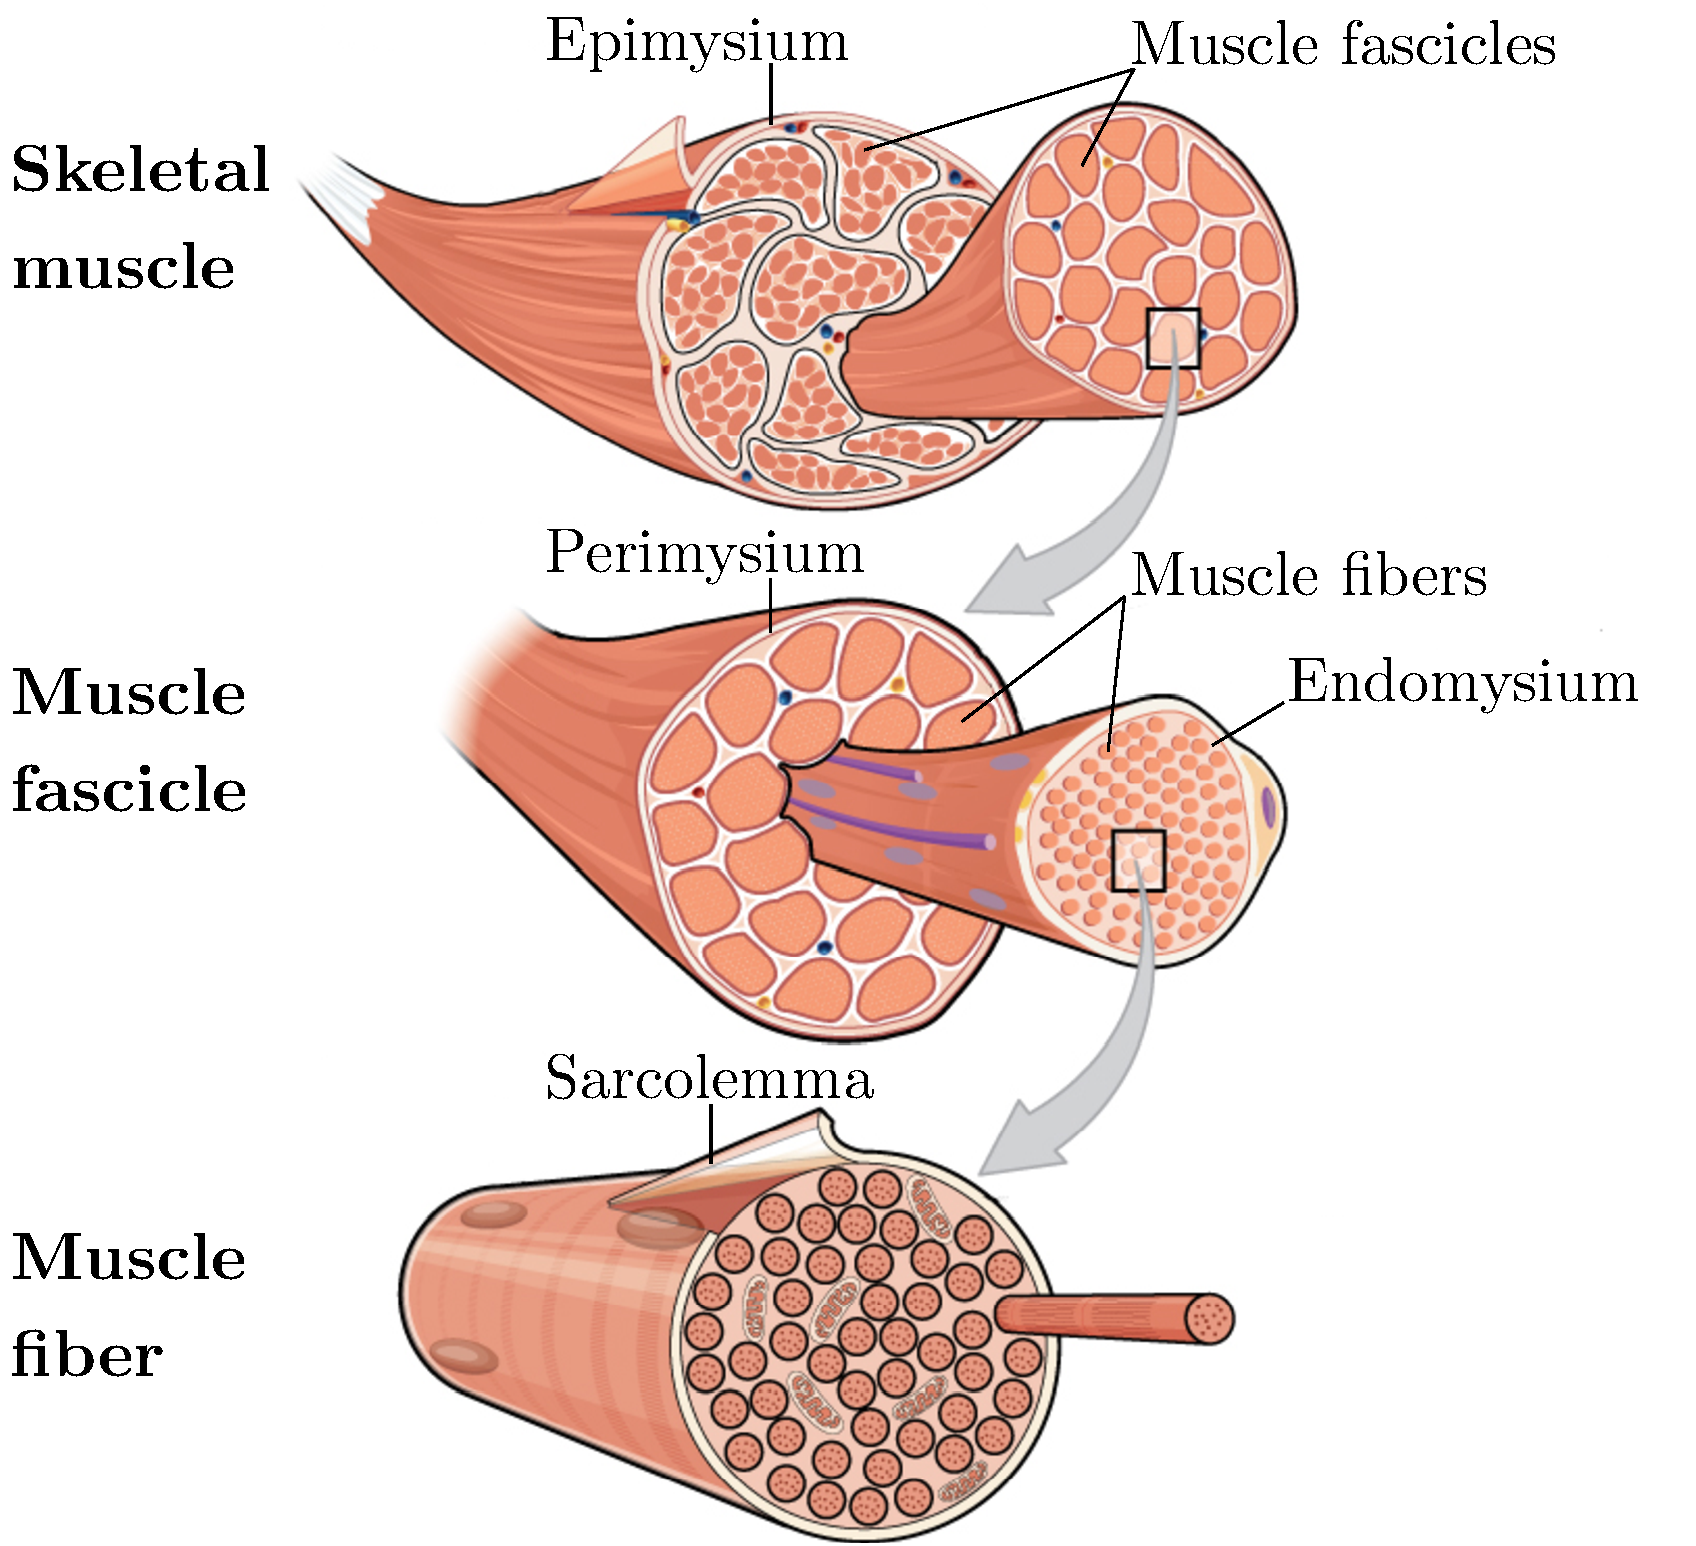
\includegraphics[scale=.4]{Figures/FIBER.pdf}
\caption[Skeletal muscle extracellular matrix]{Skeletal muscle extracellular matrix (ECM).}
\label{fig: ECM}
\end{figure}
%*********************************************************
Skeletal muscle cells (Figure~\ref{fig: ECM}) are approximately cylindrical in shape with diameters in range of 10 to $\SI{100}{\micro\meter}$ but extending up to a few centimeters in length. 
Each muscle cell (fiber) contains the contractile apparatus which is the actin-myosin complex. 
The muscle fiber contraction is itself triggered by an impulse from an axon that innervates each muscle fiber. 
The neural impulse that modulates the contraction is communicated to the axon via a motor neutron. 
Structurally, each muscle fiber is surrounded by an matrix that is largely made of macromolecules such as collagen and proteoglycan. 
This matrix is a connected hierarchical network with the endomysium surrounding each muscle fiber, the perimysium surrounding a bundle of muscle fibers (fascicles) and the epimysium, the entire muscle. 
This collagen matrix is collectively known as the extracellular matrix; typical widths of the endomysium and perimysium are a couple of microns. 
Force produced in the muscle was initially thought to be completely transmitted to the tendon via the myotendinous junction (junction of muscle fiber and tendon). 
However, evidence from prematurely terminating fibers or experiments that deliberately severed the muscle fiber-tendon junction show that there are alternate pathways, presumably through the extracellular matrix that is able to transmit the force produced by muscle fibers to the tendon. 
The mechanism by which the force generated by the muscle fiber is transmitted via the endomysium to the tendon is postulated to be through the shearing of the endomysium; this has been confirmed by computational muscle models. 
%-new paragraph-%

%-new paragraph-%
The non-invasive nature of Magnetic Resonance Imaging (MRI) renders it particularly amenable to \textit{in-vivo} longitudinal studies of aging and disuse for both research and clinical purposes. 
MRI can monitor the \textit{in-vivo} changes in MR mass (volume), muscle tissue composition (macromolecular/ connective tissue, adipose, and muscle fiber fraction), muscle architecture (muscle fiber length, pennation angle, curvature), muscle perfusion, and muscle microarchitecture (diffusion modeling). 
In addition to structural muscle imaging, dynamic MR imaging enables functional imaging: mapping of muscle deformation under different contraction paradigms. 
Spatial patterns of muscle deformation and strain can be quantified with functional muscle imaging and these maps provide an additional view into muscle performance not possible by gross measurements such as isometric muscle strength. 
%-new paragraph-%

%-new paragraph-%
Dynamic imaging of skeletal muscles using velocity encoded MR pulse sequence has been previously established in Prof. Sinha's research group and applied to lower limb muscle to study changes due to disuse atrophy. 
The developed methods revealed important information on the heterogeneity of strain along the length of the fibers, architectural gear ratio, the compliance (stiffness) of the tendon in normal and in disuse atrophy, and the asymmetry of deformation in the muscle cross-section. 
This body of work relied on one dimensional muscle/tendon strain computed along the fascicles/tendon from the velocity encoded images. 
Further, strain computation was performed at select points either along fascicles or along the tendon. 
However, muscle strain is in reality a $3 \times 3$ tensor and a spatial map of the different components of the strain tensor can potentially provide additional information on muscle kinematics. 
In particular, the strain tensor components in the fiber cross-section may provide information on the constraints to deformation (or lack of/ decrease) imposed by the extra-cellular matrix. 
Further, shear strain computed from the strain tensor may provide information that potentially could be related to muscle shear; the latter deformation has been advanced as the mechanism for lateral transmission of force via the ECM. 
The developments reported in this dissertation proceeded systematically to realize the goal of computing the 3D strain tensor \textit{in-vivo} within reasonable scan times. 
The steps are summarized in the following: 
\begin{itemize}
\item Computation of the 2D strain rate tensor from velocity encoded single slice images of the lower leg.
\item Application of this method to a cross-sectional study of young and old subjects and to a longitudinal study of subjects undergoing controlled disuse atrophy.
\item Development and implementation of a fast acquisition method and reconstruction algorithm for velocity encoded phase contrast imaging to enable multi-slice acquisition and at several levels of contraction intensity.
\item Computation of the 3D strain and strain rate tensors from multi-slice 3 directional velocity encoded images of the lower leg acquired with the accelerated pulse sequence.
\item Application of this framework to a cohort of young and old subjects at several levels of contraction.	
\end{itemize}
%-new paragraph-%

%-new paragraph-%
As stated earlier, MRI provides a wealth of structural and functional data for characterizing muscle. 
Diffusion tensor imaging provides information on diffusion (anisotropic diffusion in the case of muscle) and the direction of the largest diffusion value is used to track muscle fibers in 3D. 
Muscle fiber architecture defined by muscle fiber length, pennation angle and fiber curvature is not available from any other modality (ultrasound provides information on fiber orientation but that is routinely only available in 2D slices). 
Pennation angle refers to the angle that muscle fiber makes with the sheet-like structures called aponeneurosis from which fibers originate and terminate. 
In addition to muscle mass, fiber architecture is an important determinant of muscle force. 
Diffusion tensor imaging of skeletal muscles has been previously established as an accurate \textit{in-vivo} method for determining muscle architecture. 
Beyond the primary eigenvalue and direction, the secondary and tertiary eigenvalues potentially reflect the muscle fiber morphology in the fiber cross-section. 
While inferences have been made on fiber diameters from the secondary/tertiary eigenvalue, it should be noted that it is not possible to establish direct links to tissue microarchitecture due to the fact that the eigenvalues are mapped for image voxel contains thousands of fibers and the surrounding extracellular matrix. 
Diffusion models have been developed for brain and more recently, for muscle tissue that allow the experimentally derived diffusion eigenvalues to be fitted to an underlying physiological model of diffusion. 
My focus within the structural muscle imaging is to derive parameters that characterize tissue microstructure by utilizing two models of the diffusion in muscle. 
This effort provides information on muscle and ECM microstructure not available with other imaging approaches. 
DTI modeling included the following developments/application:
\begin{itemize}
\item Implementation of the bicompartmental diffusion model with exchange and application of this model to a longitudinal study involving diffusion tensor imaging on pre- and post- unloading induced by unilateral limb suspension (muscle disuse).
\item Development and implementation of the Stimulated Echo Echo Planar pulse sequence to allow for time dependent diffusion data acquisition.
\item Implementation of the Random Permeable Barrier Model of diffusion and application of the model to a cross-sectional study on aging.
\end{itemize}
Both functional and structural studies required extensive software development, all of the codes are publicly available, the links are provided in the relevant chapters.
%-new paragraph-%

%-new paragraph-%
The immediate goal of the Muscle Imaging and Modeling Lab under Prof. Sinha is to implement and evaluate advanced MRI techniques and to extract relevant indices for tracking changes in muscle structure and function in age and disuse atrophy. 
Knowledge gained from this will be used to develop objective biomarkers for conditions such as \textit{sarcopenia} and \textit{dynapenia} and help in characterizing these conditions, in tracking their progress, and in designing customized intervention measures. 
My contribution to this overarching goal is the development of new biomarkers of function and structure; these biomarkers will help in furthering the understanding of the pathophysiology of aging and disuse atrophy.
